\documentclass[b5paper,oneside,british,intoc,bibliograph=totoc,index=totoc,BCOR10mm,twoside,openright]{book}
\usepackage[LGR,T1]{fontenc}
%\usepackage[utf8]{inputenc}
\usepackage{inputenc}
\usepackage{fancyhdr}
\pagestyle{fancy}
\setcounter{tocdepth}{3}
\usepackage{babel}
\usepackage{float}
\usepackage{textcomp}
\usepackage{amsmath}
\usepackage{amsthm}
\usepackage{graphicx}
\usepackage{setspace}
\usepackage{subcaption}
\usepackage{csquotes}
\usepackage{pdflscape}
\usepackage{graphicx}
\usepackage[toc,page]{appendix}
\usepackage{algorithm}
\usepackage{algpseudocode}


\setstretch{1.2}
\usepackage[unicode=true,pdfusetitle,
 bookmarks=true,bookmarksnumbered=false,bookmarksopen=false,
 breaklinks=false,pdfborder={0 0 1},backref=false,colorlinks=false]
 {hyperref}
\hypersetup{
 pdfpagelayout=OneColumn, pdfnewwindow=true, pdfstartview=XYZ, plainpages=false}

\makeatletter
\g@addto@macro{\UrlBreaks}{\UrlOrds}


\newcommand*\LyXThinSpace{\,\hspace{0pt}}
\pdfpageheight\paperheight
\pdfpagewidth\paperwidth

\DeclareRobustCommand{\greektext}{%
  \fontencoding{LGR}\selectfont\def\encodingdefault{LGR}}
\DeclareRobustCommand{\textgreek}[1]{\leavevmode{\greektext #1}}
\ProvideTextCommand{\~}{LGR}[1]{\char126#1}

\providecommand{\tabularnewline}{\\}
%% A simple dot to overcome graphicx limitations
\newcommand{\lyxdot}{.}

\numberwithin{equation}{section}
\numberwithin{figure}{section}

\usepackage{amsthm,amsmath}
%\RequirePackage{hyperref}
\usepackage{graphicx}
\usepackage{rotating}
\usepackage{colortbl}
\usepackage{url}
\usepackage{siunitx}
\usepackage{algorithm}
\usepackage{algpseudocode}


\usepackage[a4,cam,center]{crop}

\usepackage{multicol}
\usepackage{listings}
\usepackage{xcolor}
\definecolor{hellgelb}{rgb}{1,1,0.9}
\definecolor{colKeys}{rgb}{0,0,1}
\definecolor{colIdentifier}{rgb}{0,0,0}
\definecolor{colComments}{rgb}{1,0,0}
\definecolor{colString}{rgb}{0,0.5,0}
\lstset{%
float=hbp,%
identifierstyle=\color{colIdentifier}, %
keywordstyle=\color{colKeys}, %
stringstyle=\color{colString}, %
commentstyle=\color{colComments}, %
columns=flexible, %
tabsize=2, %
frame=single, %
extendedchars=true, %
showspaces=false, %
showstringspaces=false, %
numbers=left, %
numberstyle={\tiny\ttfamily}, %
stepnumber=5, %
breaklines=true, %
backgroundcolor=\color{hellgelb}, %
breakautoindent=true, %
basicstyle={\small\ttfamily},%
language=C,%
captionpos=b%
}


\usepackage{fancyheadings}
\pagestyle{fancy}
\renewcommand{\chaptermark}[1]%
{\markboth{\uppercase{\thechapter.\ #1}}{}}
\renewcommand{\sectionmark}[1]%
{\markright{\uppercase{\thesection.\ #1}}}

\newcommand{\helv}{%
\fontfamily{phv}\fontseries{b}\fontsize{9}{11}\selectfont}
\lhead[\helv \thepage]{\helv \rightmark}
\rhead[\helv \leftmark]{\helv \thepage}
\cfoot{}

% non voglio sottosezioni e paragrafi nella table of content
\renewcommand\l@paragraph[2]{}
\renewcommand\l@subsubsection[2]{}

\usepackage[backend=bibtex8,style=nature]{biblatex}
\addbibresource{bibs/PhDThesisBib.bib}
\DeclareSymbolFont{extraup}{U}{zavm}{m}{n}
\DeclareMathSymbol{\varheart}{\mathalpha}{extraup}{86}


% limits underneath
\DeclareMathOperator*{\argminA}{arg\,min} % Jan Hlavacek
\DeclareMathOperator*{\argminB}{argmin}   % Jan Hlavacek
\DeclareMathOperator*{\argminC}{\arg\min}   % rbp

\newcommand{\argminD}{\arg\!\min} % AlfC

\newcommand{\argminE}{\mathop{\mathrm{argmin}}}          % ASdeL
\newcommand{\argminF}{\mathop{\mathrm{argmin}}\limits}   % ASdeL

% limits on side
\DeclareMathOperator{\argminG}{arg\,min} % Jan Hlavacek
\DeclareMathOperator{\argminH}{argmin}   % Jan Hlavacek
\newcommand{\argminI}{\mathop{\mathrm{argmin}}\nolimits} % ASdeL

\newcommand{\cs}[1]{\texttt{\symbol{`\\}#1}}

%%%%%%%%%%%%%%%%%%%%%%%%%%%%%%%%%%%%%%%%%%y

\usepackage[Lenny]{fncychap/fncychap}
\setcounter{tocdepth}{6}

\makeatother

\usepackage{listings}
\lstset{breaklines=true,
fontadjust=true,
frame=lines,
language=R,
tabsize=2}

%\startlocaldefs
\algnewcommand\algorithmicinput{\textbf{INPUT:}}
\algnewcommand\INPUT{\item[\algorithmicinput]}
\algnewcommand\algorithmicoutput{\textbf{OUTPUT:}}
\algnewcommand\OUTPUT{\item[\algorithmicoutput]}
%\endlocaldefs


\begin{document}
\pagestyle{empty}

\begin{center}
UNIVERSIT\'A DEGLI STUDI DI SALERNO
\par\end{center}

\begin{center}
DOTTORATO IN MANAGEMENT \& INFORMATION TECHNOLOGY
\par\end{center}

\bigskip{}

\begin{center}

\includegraphics[scale=0.2]{img/logoUnisa}
\par\end{center}

\bigskip{}

\begin{center}
CURRICULUM: INFORMATION SECURITY \& INNOVATION SYSTEMS
\par\end{center}

\begin{center}
COORDINATORE: Ch.mo. Prof. Antonelli Valerio
\par\end{center}

\begin{center}
Ciclo XVII N.S.
\par\end{center}

\vspace{1.5cm}

\begin{center}
Novel tools for reproducible 

Next Generation Sequencing data analysis and integration 
\par\end{center}

\vspace{1.5cm}

\textbf{\large{}Relatori}\hfill{}\textbf{\large{}Candidato}{\large \par}

Ch.mo. Prof. Tagliaferri Roberto\hfill{}Righelli Dario

Ch.mo. Prof. Angelini Claudia\hfill{}Matr. 8800800010

\vspace{1.5cm}

\begin{center}
ANNO ACCADEMICO 2017/2018
\par\end{center}

\cleardoublepage

\begin{quotation}
\begin{flushright}
\textit{
How to reach a goal? \\
Without haste but without rest\\
Goethe}
\par\end{flushright}
\end{quotation}


\cleardoublepage
% \phantomsection
\addcontentsline{toc}{chapter}{Acknowledgements}

Add acknowledgements here
%\include{acknowledgements}

\cleardoublepage

\addcontentsline{toc}{chapter}{Abstract}

Write your abstract here
\section*{Abstract}
{\setlength{\parindent}{0cm}
Massive parallel sequencing technologies are producing a vast amount of genome-wide data about cells, tissues and model organisms, useful to understand many of biological mechanisms, like protein-chromatin interactions (e.g. ChIP-Seq), DNA methylation (Methyl-Seq or BS-Seq), chromatin accessibility (e.g. Atac-Seq), global transcriptional and translational activities (e.g. RNA-Seq) and 3-D organisation of chromatin (e.g. Hi-C), giving the possibility to study same individual or experimental condition from many different points of view (transcriptomics, epigenomics, etc.) with a very high resolution. Each type of these “omic” data explains a different aspect of cellular behaviour. To give a comprehensive view of the cell regulatory mechanisms it is necessary not only to perform a single level analysis, but also to provide novel statistical and computational models for integrating different omic types within a unified study.

This thesis is focused on development of three main computational tools (\textit{ticorser}, \textit{DEScan2} and \textit{IntegrHO}), allowing data analysis and integration of multiple next generation sequencing experiments.
Additionally, a fourth tool (\textit{easyReporting}) for reproducible computational research is presented.

\textit{Ticorser} (time course RNA-seq data analyser) is a novel R package aimed to analyse time-course RNA-seq data. It offers multiple methods for differential expression data analysis and provides multiple plots useful to explore and visualize the results at each step of the analysis. Furthermore, it also provides methods for functional integration by annotating genes in pathways and GO-terms.

\textit{DEScan2} (Differential Enriched Scan 2) is a novel R package for ATAC-seq data analysis, one of the emerging techniques for investigating the chromatin accessibility. It consists in the following three-step procedure : 1) It identifies candidate regions inside each sample with a peak caller; 2) It filters out potential artefacts by aligning the candidate regions between the samples and removing those candidate regions that were not reproducible between samples 3) It produces a count matrix of regions and samples, useful for differential enrichment between multiple conditions and also for integrating this data type with other omic data, such as RNA-Seq.

\textit{IntegrHO} (Integration of High-Throughput Omics data) is a Graphical User Interface (GUI), written in R and Shiny, aimed to analyse and integrate multi-omics data types. It provides a friendly interface to the above mentioned tools, and also incorporates a wide selection of methods and other tools available in literature. This platform, through an easy point-and-click approach, enables the user to analyse and explore single omic data, such as RNA-seq, ChIP-seq and ATAC-seq and, moreover, it offers the possibility to integrate them at different levels, such as gene-peak annotation and functional annotation methods.

\textit{EasyReporting} is an R package for an automatic report creation (easyreporting), developed to address the problem of reproducibility of a computational analysis.  
Thanks to the R6 class paradigm on which is based on, it is easy to use and to extend.

Overall, this work proposes and combines several computational tools for properly analysing, visualizing, comparing, integrating and tracing different types of omics data.
}

\hypersetup{hidelinks} % to hide suares around links

\pagestyle{plain}\tableofcontents

\cleardoublepage{}
\pagestyle{fancy}


%\include{original_articles}
\newpage
\chapter{Introduction}
This chapter provides all the aspects needed to understand the context of this thesis work, highlighting, moreover, which are the the proposed goals of it.
%explains some basic information useful to understand the context where this thesis work has been developed.

It starts from showing some biological basic aspects and how it is possible to study some cellular behaviours from multiple points of view, using different sequencing techniques and how to integrate them.
Showing, moreover, the importance of keeping trace of the processes involved in the information extraction and why we underlying this aspect. 



\section{Biological Background}
\subsection{The cell}
\label{sec:cell}
Cells are the fundamental units of every living being, which can be made up of one cell (unicellular) or more (multicellular).
Indipendently on how big and complex an organism could be, each cell always maintains its individuality and its independence, but maintaining common structural proprieties.

The internal volume is defined by the \textit{cytoplasm}, which is a liquid solution where several insoluble particles stands, such as enzimes, \textit{RNA} and metabolites.
Moreover, it is possible to distinguish multiple organelles, such as \textit{ribosomes}, the \textit{endoplasmic reticulum}, the \textit{golgi comples},\textit{lisosomes} and the \textit{nucleus} (figure \ref{fig:cell}).
In particular, this last one has a the role of contain the genome, represented by the \textit{DNA}.

\begin{figure}[h]
\centering
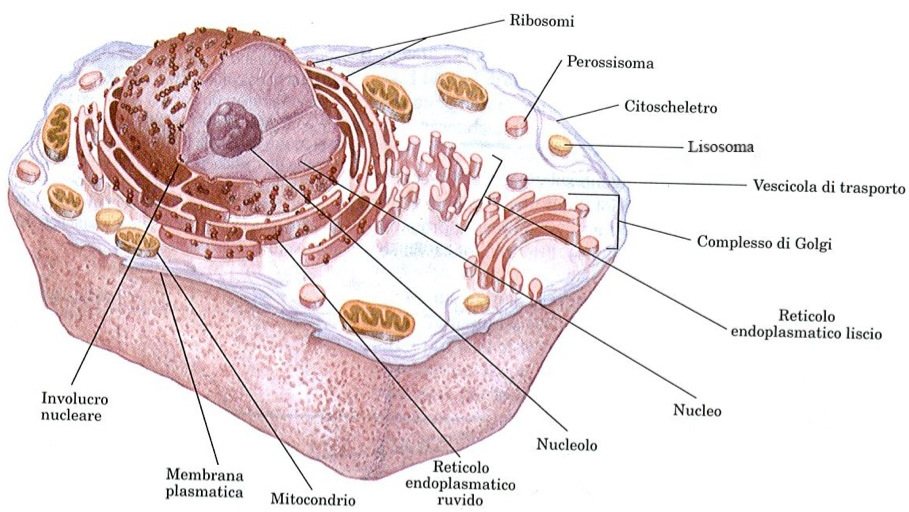
\includegraphics[width=10cm, keepaspectratio]{img/intro/cell.png}
\caption[The Cell]{Schematic representation of a cell.}
\label{fig:cell}
\end{figure}

\subsection{The DNA}
\label{sec:genica}
The \textit{DNA} was been isolated for the first time by the German doctor Friederick Miescher in 1869, while in the same decade the English biologist Charles Darwin was publishing \textit{On the Origin of the Species} and the  Augustinian friar scientist was communicating his results on the pees to the Brunn Natural History Society.

Because the substance isolated by Miescher was white, lightly acid and present only into the cells nuclei, it was been termed \textit{Nucleic Acid}.
Name modified afterwards in \gls{dna}, to distinguish is from the another one, very similar, the \gls{rna}.

These two molecules are constituted by \textit{nucleotides}, constituted by a nitrogen base, deoxyribose sugar and a phosphate group.
We distinguish two nitrogen bases, purines and pyrimidines.
Inside the \gls{dna}, we have two \textit{pyrimidines}, \textit{adenine (A)} and \textit{guanine (G)}, and two \textit{pyrimidines}, the \textit{Cytosine (C)} and the \textit{Thimine (T)}  .
Inside \gls{rna} \textit{Thymine} is substituted by the \textit{Uracil (U)}.

\begin{figure}[h]
\centering
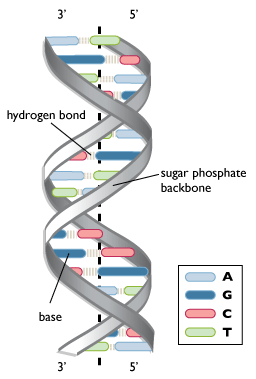
\includegraphics[width=5cm, keepaspectratio]{img/intro/dna1.png}
\caption[the \gls{dna}]{Schematic representation of double-stranded filament structure of \gls{dna}. The legend report the four nitrogen bases, Adenine, Guanine, Cytosine and Thymine.}
\label{fig:dna}
\end{figure}

\gls{dna} structure (figure \ref{fig:dna}) was discovered, in the 50's, by the American scientist James Watson, the French physicist Francis Crick and the English chemist-physicist Rosalind Franklyn.
According to their model the \gls{dna} is a double-stranded filament, where Adenines can pair only with Thymines and Guanines only with Cytosines.
The four bases constitute the alphabet for the genetic message.

\gls{dna} is folded on itself (\textit{\gls{dna} packaging}, thanks to specific "beads" called \textit{nucleosomes}, which themselves consist of eight proteins with tails, called \textit{histones}, that have the \gls{dna} wrapped on them.
This mechanism enables to store around 2 meters of chromatin inside a nucleus of a 2-10 micron diameter, when referring to Human specie.

Moreover, the \gls{dna} contains the \textit{genes}, particular sections containing relevant information for building proteins and other fundamental molecules for the cellular behavior regulation.
Each gene is localized on a precise position of a \textit{Chromosome}, which are in different number for each specie.
Each chromosome is constituted by \gls{dna} within thousands genes.

\begin{figure}[h]
\centering
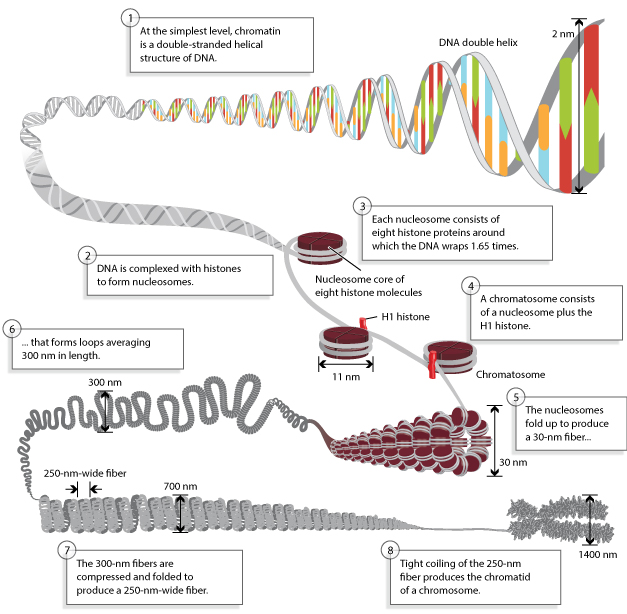
\includegraphics[width=8cm, keepaspectratio]{img/intro/dna2.jpg}
\caption[Chromosomes and \gls{dna}]{Representation of the relation between \gls{dna} and Chromosomes.
Inside the cell nucleus there are pairs of chromosome, constituted by chromatin, which fundamental unit is constituted by nucleosomes, on which the \gls{dna} is wrapped around, containing the genetic information in gene form. (image adapted from \cite{Annunziato2008})}
\label{fig:dnachromosome}
\end{figure}

Figure \ref{fig:dnachromosome} better helps  to understand the relationship between chromosomes, chromatin, nucleosomes and genes.

It is important to underlying that since some decades ago the Central Dogma of Molecular Biology was founded on the transcription - translation principle, where \gls{dna} was transcribed in \gls{rna}, which subsequently it would have been translated into protein.

Nowadays, we know that the gene transcription is regulated by several mechanisms, and moreover, the translation is not the only process fated for \gls{rna}.

Indeed, for a transcription of a gene, there are some requisites to be respected, such as the accessible of that specific part of the chromatin, or the binding of specific proteins enabling the accession to the gene region, or the histone modification processes, such as \textit{Acetylation}, \textit{Methylation}, \textit{Phosphorylation}, and others, which modifies the state of specific histones, and influencing gene expression regulation. 
  
\begin{figure}[h]
\centering
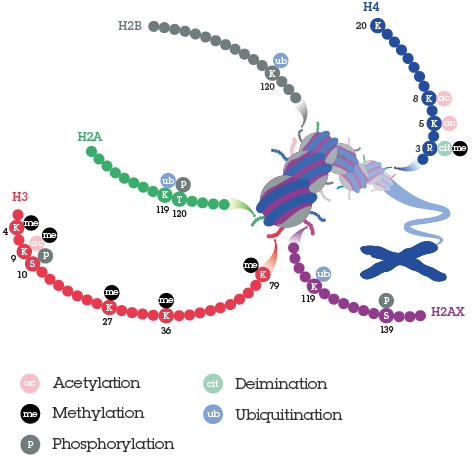
\includegraphics[width=8cm, keepaspectratio]{img/intro/hm.png}
\caption[Histon modification]{Representation of some processes involved in histone modification, influencing gene expression regulation.}
\label{fig:histmod}
\end{figure}


\section{Sequencing Techniques}
\input{sections/general_seqs.tex}

\subsection{RNA-Seq}
proviamo a scrivere qualcosa


\subsection{ChIP-Seq}
\input{sections/chipseq.tex}

\subsection{Atac-Seq}
\input{sections/atacseq.tex}

\subsection{Other Sequencing Tecniques}
\input{sections/otherseqs.tex}

\section{Data Analysis}
\input{sections/dataanal.tex}

\subsection{RNA-Seq Methods}
\input{sections/rnaanal.tex}

\subsection{ChIP-Seq Methods}
\input{sections/chipanal.tex}

\subsection{Atac-Seq Methods}
\input{sections/atacanal.tex}

\section{Integration}
All above-mentioned sequencing techniques are aimed to investigate only one cellular compartment at a time, but in order to obtain a more comprehensive view of the cellular behaviour, it is necessary to look at more than one omics at the same time.

\begin{figure}[H]
\centering
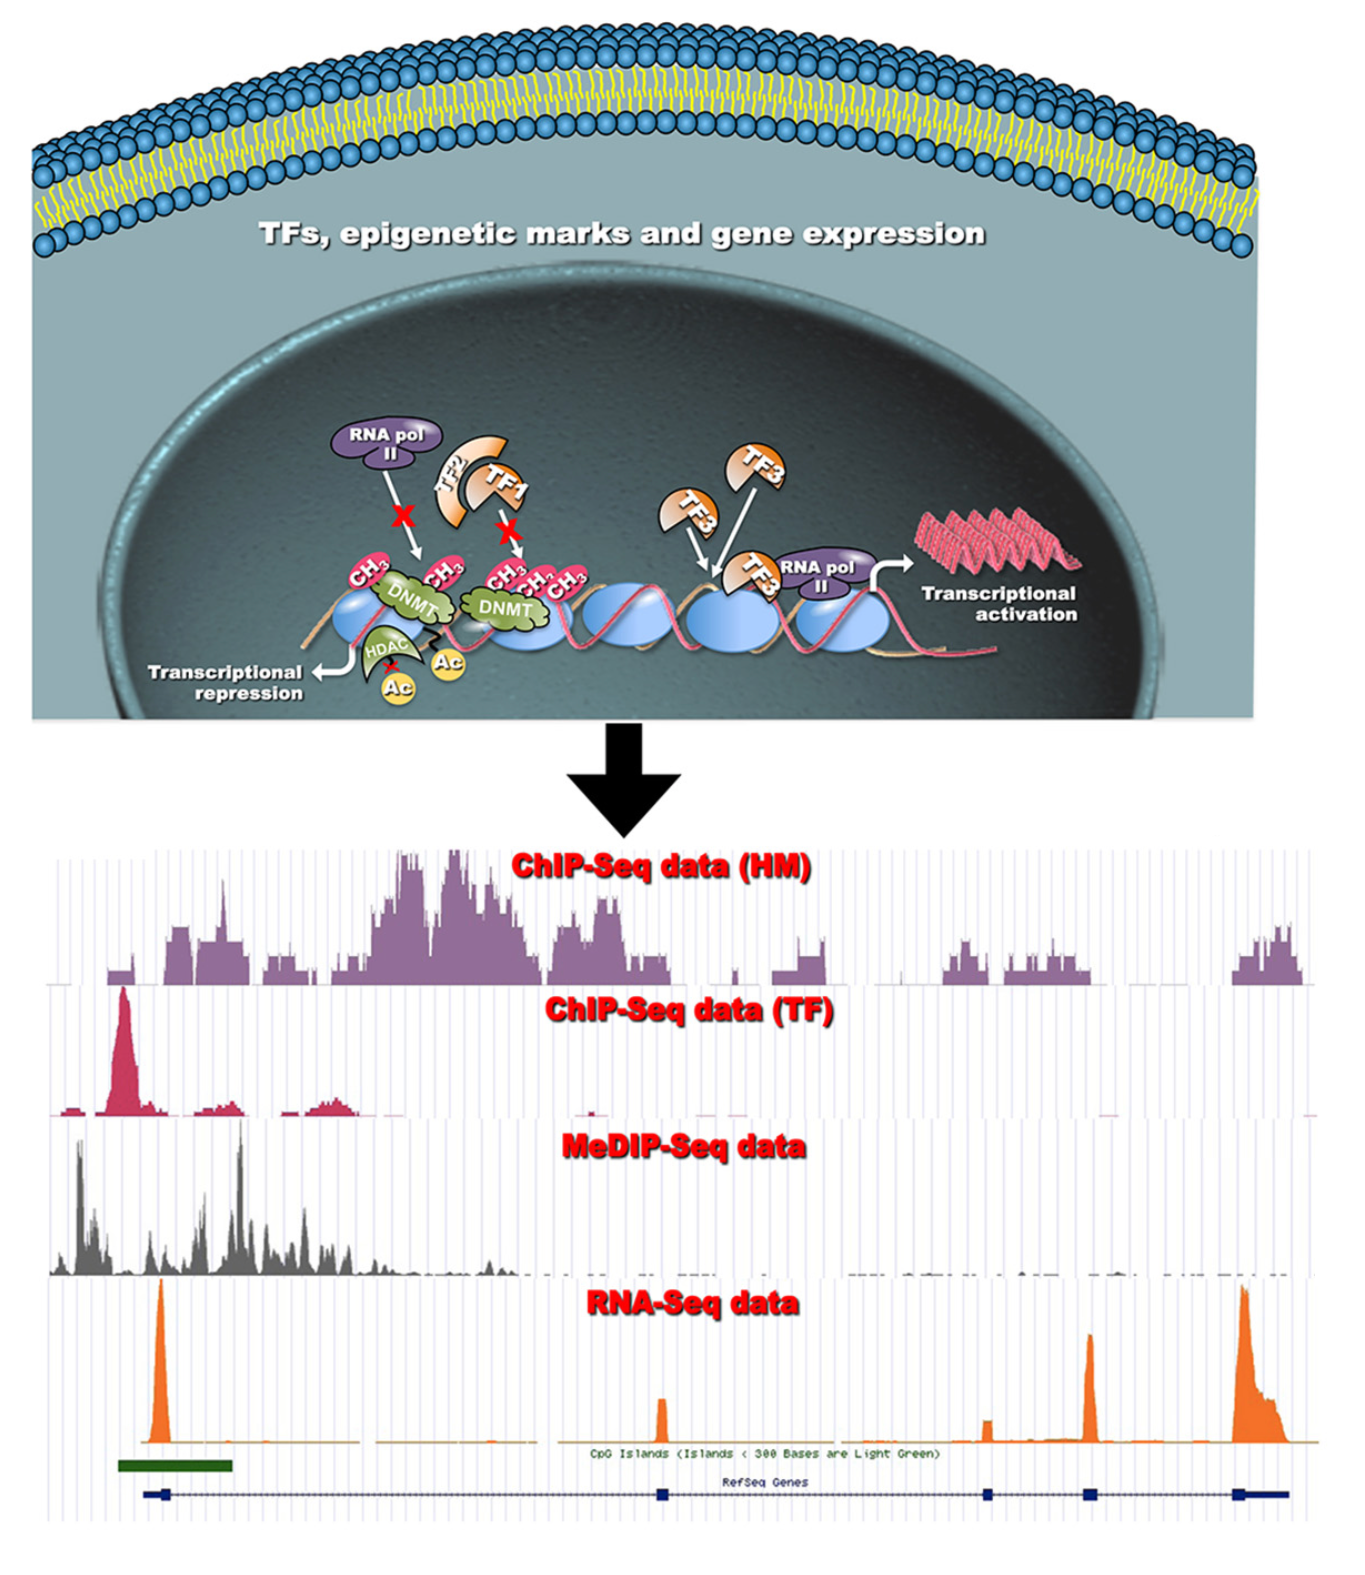
\includegraphics[width=9cm, keepaspectratio]{img/intro/multiomicsex.png}
\caption[Multi-Omics Representation]{An example of different omics coming from the same biological representation. (adapted from \cite{Angelini2014c})}
\label{fig:omics}
\end{figure}

Indeed, we can imagine each omics as a camera in a multi-view camera system pointed on a building from different points of view.
Each device takes snapshots of the building from different angles, but the information is still fragmented.
In order to reconstruct a 3D model of the building, we need to put each device snapshots together.

\begin{figure}[h]
\centering
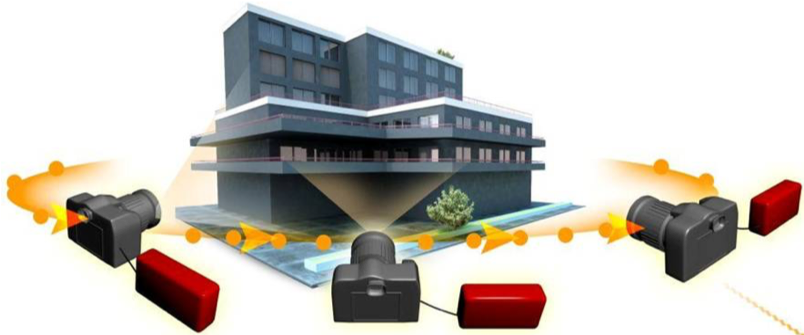
\includegraphics[width=8cm, keepaspectratio]{img/intro/cameras.png}
\caption[Integration cameras]{An illustrative exaple of a multi-view camera system pointed on a building.}
\label{fig:cameras}
\end{figure}

The same idea can be adapted to the sequencing techniques, we need to integrate the information coming from different omics in order reconstruct (and understand) how multiple mechanisms orchestrate the cellular behaviour.

Indeed, we can imagine a typical combination of epigenomics factors affecting the chromatin in order to influence the transcription of one or more genes.
An \glspl{hm} (such as \textit{Acetylation}) can have inhibited the accession to bind specific nucleosomes, because already occupied by specific \glspl{tf}, inhibiting, in such a way, the expression of those genes present in that particular portion of the chromatin (upper part of figure \ref{fig:omics}).
To investigate these processes, we can perform multiple experiments of \textit{RNA-seq} and \textit{ChIP-seq} (one for the \gls{hm} and one for the \textit{tf}) to study singularly each epigenomics factors and the gene expression (lower part of figure \ref{fig:omics}). 

As figure \ref{fig:funnell} outlines, multi-omics data integration can be made at different levels, by graphical exploration, by functional annotation, by network fusion and by dimensionality reduction.
We can distinguish two main approaches,; ''analyze each omics then integrate the results'' and ''jointly analyze each omics to improve the power''.
The first one can be done also with few samples, where each omics is analyzed standalone and then the results can be combined to obtain a common response (levels 1 and 2 of figure \ref{fig:funnell}).
The second main approach needs a high number of samples to analyze all the omics together to obtain more power in the response prediction (levels 3 and 4 of figure \ref{fig:funnell}) \cite{Rohart2017, Argelaguet2018, Jia2017, Meng2016}.

\begin{figure}[h]
\centering
\includegraphics[width=8cm, keepaspectratio]{img/intro/funnell.pdf}
\caption[Integration Funnell]{A schematic representation of multi-omic data integration levels.
}
\label{fig:funnell}
\end{figure}

More in general, integration can be performed at different levels (i.e. descriptive, exploratory, inferencial, etc.).

With graphical exploration, we can visualize data coming from different sources (e.g. \textit{RNA-seq} and \textit{ChIP-seq}) using specific tools designed at this scope, such as \textit{Genome Browser} \cite{Karolchik2011} or \gls{igv} \cite{Robinson2011, Thorvaldsdottir2013} and looking to the overlapping regions, or where expressed epigenomic markers have corrispondence with gene expression sites.

We refer to functional annotation integration when using methods combining analysis results (such as relevant lists of genes) with publicly available databases,  like the Gene Ontology\footnote{http://www.geneontology.org/} and pathway (\textit{KEGG}\footnote{https://www.genome.jp/kegg/} or \textit{Reactome}\footnote{https://reactome.org/}) based ones, to detect functional responses highly related to the experimental condition under investigation.

It is possible to integrate multiple omics data types by constructing multiple regulation networks, one for each omic analyzed, and then combine these networks with fusion techniques.
This integration aspect is used when a high number of data samples is available or when having multiple-omics data types coming from the same patients \cite{Wang2014}.

A deeper level of integration is achievable with dimensionality reduction techniques. 
Also in this case, several samples are needed to be able to obtain relevant and reliable results.
Generally speaking, these methods are able to start from multiple samples coming from different omics and to reduce their dimensionality, enabling to identify common cellular behavioural aspects \cite{Rohart2017, Argelaguet2018}.





\subsection{Low Level Integration}
\input{sections/lowlevintegr.tex}

\subsection{High Level Integration}
\input{sections/highlevintegr.tex}

\section{Reproducible Computational Research}
\input{sections/reprcompres.tex}

\chapter{Methods}
Here we present \textit{easyReporting}, an \textit{R6} \footnote{\url{https://adv-r.hadley.nz/r6.html}}\footnote{\url{https://cran.r-project.org/web/packages/R6/index.html}} class\footnote{\url{https://en.wikipedia.org/wiki/Class_(computer_programming)}} developers to integrate a reproducible research layer inside their software products, as well as lazy analysts to speed up their report production without learning the \textit{rmarkdown} language.

In such a way, thanks to minimal additional efforts of developers, the end user has available an \textit{rmarkdown} file within all the source code generated during the analysis, divided into \glspl{cc} ready for the compilation.

Once manually edited with comments and descriptions the file can be compiled to produce an enriched document within input data, source code and output results.

A so final document can be attached to the publication of the analysis as supplementary material, helping the interested community to entirely reproduce the computational part of work (figure \ref{fig:rrscheme}). 

The package is accessible at the following link:\\ \href{https://github.com/drighelli/easyreporting}{https://github.com/drighelli/easyreporting} 

\subsubsection{General Description and Initialization}

The class can to be imagined as a schematic representation of the \textit{rmarkdown} file (\textit{report}), indeed 
its attributes represent the \textit{report} characteristics, which are typically inserted in the header of the file.
But our class methods are not only for the attributes manipulations but also for insertion of \glspl{cc}, comments and section titles inside the \textit{report}.

As any typical class, before of using it, \textit{easyReporting} requires to be initialized with the \lstinline!new! command, passing as mandatory arguments the \textit{path} and the name of the file as \lstinline!filenamepath! and a title as \lstinline!mainTitle!.
Additionally, an \lstinline!author! and the \lstinline!documentType! can be specified.

When initializing, the class automatically creates the \textit{report} with the entire specified folder tree, setting up the header of it and declaring the general options for the \textit{rmarkdown} file.
If \textit{rmarkdown} personal options (see figure \ref{fig:knitropts} for a list of available options) are required, before creating an instance of the class, it is possible to use the \lstinline!makeOptionsList! function, and then assigning the output to the \lstinline!optionsList! argument of the class \lstinline!constructor!.

\begin{figure}[H]
\centering
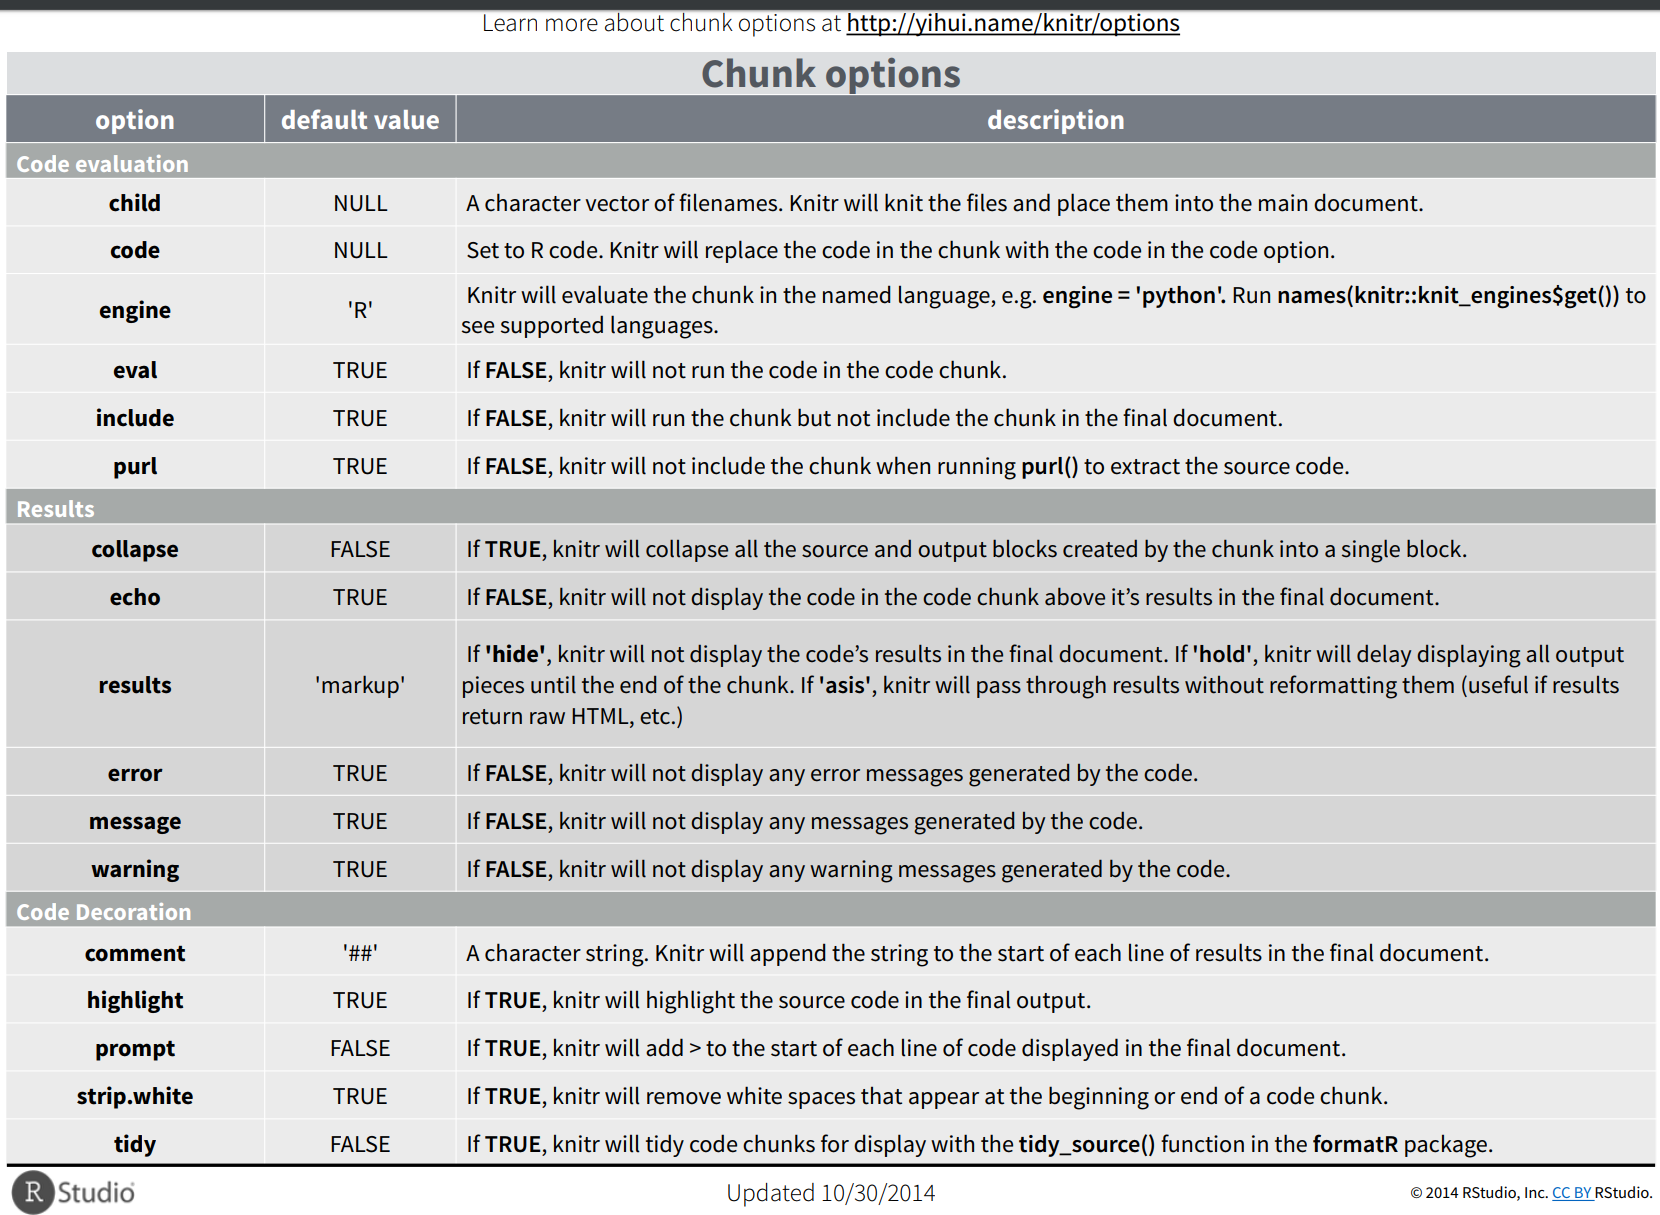
\includegraphics[width=\textwidth, keepaspectratio]{img/rr/knitropts.png}
\caption[knitr options]{A schematic table of options available using knitr and rmarkdown packages.}
\label{fig:knitropts}
\end{figure}


\subsubsection{Class Methods}

The class is provided of several methods for \textit{rmarkdown} \gls{cc} construction.

Once an \textit{easyReporting} instance is available, with \lstinline!mkdTitle! it is possible to insert six levels of titles, by setting the parameters \lstinline!title! and \lstinline!level!.
It is also possible to add natural language comments with \lstinline!mkdGeneralMsg!.

When working with \glspl{cc}, two main choices are available.
The first one gives the possibility to construct a \gls{cc} as additional steps, by using first the \lstinline!mkdCodeChunkSt!, then adding variable assignment and/or function calling with \lstinline!mkdVariableAssignment! or \lstinline!mkdGeneralMsg!, and finally closing the \gls{cc} with \lstinline!mkdCodeChunkEnd!.

In particular, when starting a \gls{cc} with \lstinline!mkdCodeChunkSt!, it is possible to assign a specific \lstinline!optionList! and/or a \lstinline!source.files.list! to be added to that \gls{cc}.

Otherwise it is possible to create an entire \gls{cc} just with \lstinline!mkdCodeChunkComplete! and assigning the entire function call as a \lstinline!message!.
This way of working is really useful with \lstinline!function! creation, where inside a developed function a simple recursive call with parameters assignment can be done as a single \lstinline!message!.






\section{TiCoRSe - Time Course RNA-Seq data analysis}
\input{sections/ticorsemethods.tex}

\section{DEScan2 - Differential Enriched Scan 2}
\input{sections/descanmethods.tex}

\section{IntegrHO - Integration of High-Throughtput Omics data}
\input{sections/integrhomethods.tex}

\chapter{Results}
\section{TiCoRSe - Time Course RNA-Seq data analysis}
\section{DEScan2 - Differential Enriched Scan 2}
\section{IntegrHO - Integration of High-Throughtput Omics data}

\chapter{Future Works}

\chapter{Conclusions}

\begin{appendices}
\include{appendixA}
%\include{appendixB}
%\include{appendixC}
\end{appendices}

%This chapter provides all the aspects needed to understand the context of this thesis work, highlighting, moreover, which are the the proposed goals of it.
%explains some basic information useful to understand the context where this thesis work has been developed.

It starts from showing some biological basic aspects and how it is possible to study some cellular behaviours from multiple points of view, using different sequencing techniques and how to integrate them.
Showing, moreover, the importance of keeping trace of the processes involved in the information extraction and why we underlying this aspect. 


%\include{aim_of_the_study}
%\include{MVDA}
%\include{INSIdEnano}
%\include{discussion}
%\include{conclusion}

%\begin{appendices}
%\include{appendixA}
%\include{appendixB}
%\include{appendixC}
%\end{appendices}

\printbibliography[heading=bibnumbered]

\cleardoublepage
% \phantomsection
\addcontentsline{toc}{chapter}{\listfigurename}
\listoffigures

\cleardoublepage
% \phantomsection
\addcontentsline{toc}{chapter}{\listtablename}
\listoftables

%\listoffigures
%\listoftables

\end{document}